\documentclass{article}
\setlength{\topsep}{0 in}
\setlength{\partopsep}{0 in}
\setlength{\parskip}{1.5 ex}
\setlength{\topmargin}{-.7 in}
\setlength{\oddsidemargin}{0 in}
\setlength{\textheight}{9.4 in}
\setlength{\textwidth}{6.5 in}
\setlength{\parindent}{0 in}

\usepackage[pdftex]{graphicx}
\usepackage{amssymb}
\usepackage{amsthm}
\usepackage{amsmath}
\usepackage{fourier}
\usepackage{float}
\usepackage{tikz}

\usepackage{algorithm,algpseudocode}
\newcommand{\algorithmicbreak}{\textbf{break}}
\newcommand{\Break}{\State \algorithmicbreak}
\newcommand{\algorithmiccontinue}{\textbf{continue}}
\newcommand{\Continue}{\State \algorithmiccontinue}
\newcommand{\AlgAnd}{\textbf{and}}
\algtext*{EndIf}% Remove "end if" text

\usepackage{caption}
\usepackage{multicol}
\usepackage{tikz}

\theoremstyle{definition}
\newtheorem{exercise}{Exercise}%[section]
\newtheorem{example}{Example}%[section]
\newtheorem{question}{Question}%[section]

\DeclareRobustCommand{\bigO}{%
  \text{\usefont{OMS}{cmsy}{m}{n}O}%
}

\usepackage{titlesec}
\titlespacing\section{0pt}{10pt plus 2pt minus 2pt}{0pt plus 2pt minus 2pt}
\titlespacing\subsection{0pt}{10pt plus 2pt minus 2pt}{0pt plus 2pt minus 2pt}

\begin{document}
\pagestyle{empty}

\title{}
\date{}

\captionsetup[figure]{labelFormat=empty}% redefines the caption setup of the figures environment in the beamer class.

\Large
\begin{center}
\textbf{\newline CS 577: Induction Supplemental Handout}
\end{center}

\normalsize

\subsection*{Overview}
The purpose of this handout is to contextualize induction with an example problem, explaining the steps to problem solving in detail.

Induction is a tool for mathematical proofs allowing you to prove a statement is true for any value of $n$, where $n$ is some variable within the statement. A good analogy for an inductive proof is climbing a ladder, where you want to show you can reach rung number $n$ of the ladder. First, you prove that the statement is true for some base case $n = \texttt{base\_case\_value}$ (you can step onto the bottom rung of the ladder from the ground). Then you prove that if the statement is true for $n = k$, it must be true for $n = k+1$ (if you're already on a ladder rung, you're capable of getting to the next rung, i.e. you know how to climb the ladder). In this way, you've shown that the statement is true for any value of $n \geq \texttt{base\_case\_value}$ (you can reach any ladder rung).

\begin{figure}[h]
	\centering
    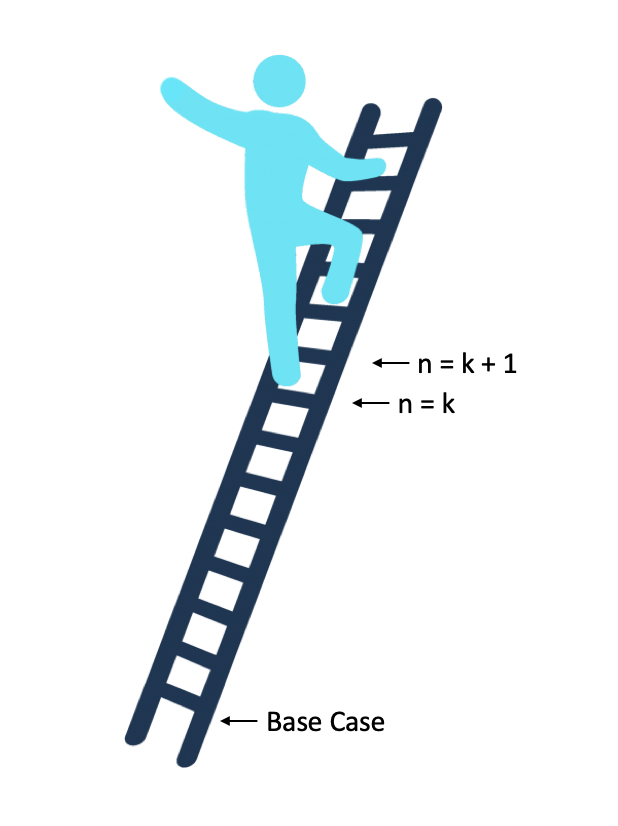
\includegraphics[width=0.5\linewidth]{ladder-induction.png}
    \captionsetup{labelformat=empty}
    \captionsetup{width=0.7\linewidth}
    \caption{Analogy for a weak inductive proof. The base case proves that you can step onto the bottom rung. The inductive hypothesis assumes that you can reach rung $k$. In  the inductive step, we prove that if you can reach rung $k$, then you can step to rung $k+1$. Together, these statements prove that you can reach any rung of the ladder.}
    \label{fig:laddder-induction}
\end{figure}

\subsection*{Strong Induction}
Strong induction uses a stronger inductive hypothesis than weak induction (described above). In a weak inductive proof our inductive hypothesis is that the statement holds for $n=k$. In a strong inductive proof, our inductive hypothesis is that  the statement holds for $\texttt{lowest\_base\_case\_value} \leq n \leq k$. A strong inductive hypothesis gives you strictly more tools in your tool belt for use in the inductive step (proving that the statement holds for $n=k+1$). 

Because your inductive hypothesis is strictly stronger than in weak induction, any inductive step that works with a weak inductive hypothesis is still valid with a strong inductive hypothesis. 

The converse is not true. For example, assume you need to have your feet on rung $k-1$ and your hands on rung $k$ in order to reach the next rung. Your inductive step states ``if I can reach rung $k-1$ and rung $k$ then I can reach rung $k+1$. I can reach rung $k-1$ and rung $k$ by the inductive hypothesis.'' This inductive step would not work in weak induction because the inductive hypothesis wouldn't be applicable to rung $k-1$. Since the strong inductive hypothesis is strictly stronger than the weak inductive hypothesis, unless the problem statement specifies that you must use weak induction, you may as well use strong induction.

\begin{figure}[h]
	\centering
    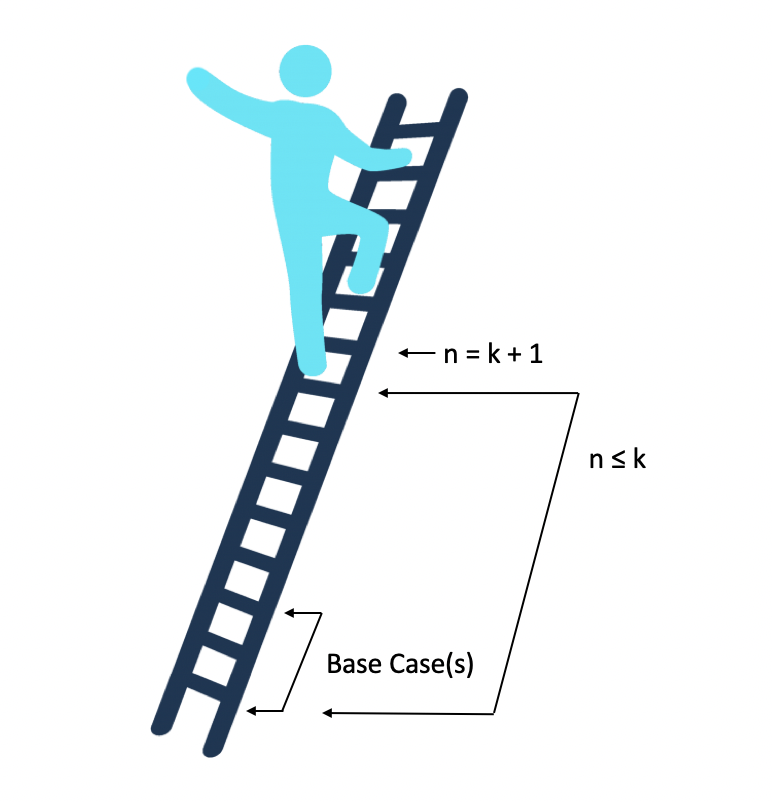
\includegraphics[width=0.5\linewidth]{strong-induction.png}
    \captionsetup{labelformat=empty}
    \captionsetup{width=0.7\linewidth}
    \caption{Analogy for a strong inductive proof. The base case proves that you can step onto the bottom rung(s). The inductive hypothesis assumes that you can reach all rungs from the base case to rung $k$ (inclusive). In the inductive step, we prove that if you assume the inductive hypothesis, then you can reach rung $k+1$. Together, these statements prove that you can reach any rung of the ladder.}
    \label{fig:laddder-induction}
\end{figure}

\subsection*{Example Problem: Making Change}
Problem statement: Prove that every value $n \geq 4$ cents can be formed from some number of 2 and 5 cent coins.

\subsection*{Step 1: What are we trying to prove? What are we inducting on?}
The first step to an inductive proof is clearly stating what we want to prove and deciding what value we will induct on. In many problems, there will be only one variable, so it will be clear what to induct on. However, in some problems, particularly in inductive proofs on graphs, there will be multiple variables that you could induct on. 

In the example problem, we want to prove that any number of cents greater than or equal to 4 can be formed by some number of 2 and 5 cent  coins. In this problem there is only one variable, so we will induct over the total value we want to make change for, $n$. 

\subsection*{Step 2: Base Case(s)}
Induction is like setting off a row of dominoes; even if the dominoes are set up so that each domino would hit the next if it fell, none of the dominoes will fall until the first one is pushed. In our inductive proof, the base case is the first domino. 

In a weak inductive proof, you only look back one rung during the inductive step. So, you only need one base case (knowing that you can reach the first rung is enough to prove that you can reach the second rung). In a strong inductive proof, you are allowed to look back at any rung before the $k+1$st in order to prove that you can reach the $k+1$st rung. Because of this, you may need multiple base cases. As before, assume your inductive step states ``if I can reach both rung $k-1$ and rung $k$, then I can reach rung $k+1$. I can reach rung $k$ and rung $k+1$ by the inductive hypothesis.'' In this scenario, if your base case was merely that you can reach the first rung, it wouldn't be enough to prove anything further. Instead, if your base cases include both the first and second rung, then you can use those two rungs to prove you can reach the third rung (and so on). In order to determine how many base cases you need, think about how many steps back you will look in the inductive step (you can always add base cases later if you need to adjust).

In the case of the coin problem, we will use strong induction. We want to have two base cases because we can always make change for a value of $n$ if we can make change for a value of $n-2$ (by adding a 2 cent coin). Having two base cases means that we will have already proven the $n-2$ case when using the inductive step.

\subsection*{Step 3: Inductive Hypothesis}
The inductive hypothesis is when we \textit{assume} that the statement we want to prove holds for $n=k$ (in weak induction) or $\texttt{lowest\_base\_case\_value} \leq n \leq k$ (in strong induction).

For our example problem, our inductive hypothesis is that we can make change for all values of $n$ such that $4 \leq n \leq k$ using only 2 and 5 cent coins.

\subsection*{Step 4: Inductive Step}
In the inductive step, we prove that the statement holds for $n=k+1$ under the assumption of the inductive hypothesis. Note that the inductive step applies to values of $n$ after the base cases, so we can assume that $k+1 > \texttt{highest\_base\_case\_value}$. \textbf{You must reference the inductive hypothesis in the inductive step.}

My recommendation is to first explicitly write out what you want to show. Not only does this help keep the goal in mind, but sometimes it can help you reverse engineer the proof, giving you insight about where to start. In the example problem, we want to show that we can make change for the value $k+1$ using only 2 and 5 cent coins.

Now we need to find a way to apply the inductive hypothesis. If you're ever stuck on where to start, try to manipulate the $k+1$ situation until you have a $k$ situation you can apply the inductive hypothesis to. For the coin problem, we want to consider a value that is less than or equal to $k$ so that we can apply the inductive hypothesis. First, let's put a 2 cent piece in the pile of change. Now  we only need to make change for the value $(k+1)-2=k-1$, which we can do \textbf{by the inductive hypothesis}. In total, we've now made change for the value $k+1$ using only 2 and 5 cent coins. Therefore, the statement we want to prove holds true for $n=k+1$.

If you're using strong induction, it's a good idea to check that you have enough base cases. In this example, the first value that's not covered by base cases is $n=6$. We set put a 2 cent piece in the pile of change and have 4 cents remaining. Because $n=4$ was covered in our base cases, we know we have enough base cases.

At this point we are done. Because we've proved that the statement holds for $n=4$ and $n=5$ and that if the statement holds for $4 \leq n \leq k$ then the statement holds for $n=k+1$, we've proven that the statement (ability to make change using only 2 and 5 cent coins) holds for all values $n \geq 4$. 

\subsection*{Structural Induction}
Structural Induction is in essence the same as mathematical induction, but applied to a recursively-defined structure rather than the set of integers. Structural induction problems ask you to prove that some proposition holds true for all objects  of a certain recursively-defined structure. My biggest tip for structural induction is to be careful about what is true (the definition of the structure), what you are assuming to be true (the inductive hypothesis), and what you want to prove (in the inductive step). Because the structure is defined recursively (and mathematically), it is easy to get mixed up on what is part of the definition and what you're trying to prove. 

Here is an example of a structural induction problem along with the solution. Note that this problem requires two inductive proofs because we are proving an iff relation. Within each section, pay close attention to the direction in each step and what we assume versus what we prove. It can helpful to double check that you are proving the correct direction during each step of the structural inductive proof.

\textbf{Problem Statement} \\
Let \textit{S} be a set recursively defined as follows: \\
Base case: $4 \in S$ \\
Recursive rule: if $x \in S$, then $x^2 \in S$.

Prove that $S$ can be equivalently defined as $x \in S$ iff $x = 4^{(2^j)}$ with some non-negative integer $j$.

\textbf{Direction 1}: if $x \in S$ then $x = 4^{(2^j)}$ for some non-negative integer $j$ \\
\textit{Base case:} Here we take the first element $x \in S$. This is $x = 4$. $4 = 4^{(2^0)}$. \\
\textit{Inductive hypothesis:} For some element $x = k \in S$, $x = 4^{(2^j)}$ with some non-negative integer $j$. \\
\textit{Inductive step:} We want to show a property about $y$, the next element in $S$ after $x = k$. Namely, we want to show that $y = 4^{(2^m)}$ for some non-negative integer $m$. \\
By the recursive definition, $y = x^2 = k^2$. Note that in mathematical induction, we would consider $k+1$. In the case of structural induction, because we're inducting over the structure $S$, we consider the next element in the set rather than simply $k+1$. \\
$y = k^2$. By the inductive hypothesis, $y = (4^{(2^j)})^2 = 4^{((2^j)(2))} = 4^{(2^{(j+1)})} = 4^{(2^m)}.$

\textbf{Direction 2:} if $x = 4^{(2^j)}$ for some non-negative integer $j$ then $x \in S$ \\
\textit{Base case:} Here we take the first possible value of $x = 4^{(2^j)}$. Because $j$ must be a non-negative integer, the base case is $j=0$. $x = 4^{(2^0)} = 4^1 = 4 \in S$ from the base case rule in the definition of $S$. \\
\textit{Inductive hypothesis:} For some value $j=k$, x = $4^{(2^k)} \in S$. \\
\textit{Inductive step:} Note that in this direction, we're inducting over the integer $j$ and proving that the corresponding value $x \in S$ (rather than inducting over elements $x$ in the set $S$ and showing that $x$ can be defined according the closed form $x=4^{(2^j)})$. In the inductive step we will consider the value of $x$ associated with  $j=k+1$. We want to show that $x=4^{(2^(k+1))} \in S$. \\
$x = 4^{(2^{(k+1)})} = 4^{[(2^k)(2)]} = (4^{(2^k)})^2$. By the IH, $y = 4^{(2^k)} \in S$. By the recursive definition of $S$, since $x = y^2$ and $y \in S$, $x \in S$.

\subsection*{Graph Induction}
The biggest tip for graph induction is that -- unless you are using structural induction -- you want to \textit{break down rather than build up} during the inductive step. This means that your inductive step should begin with the $k+1$ case, remove things from the graph until you have a $k$ case (you must demonstrate that this is always possible), apply the inductive  hypothesis to the $k$ case, put what you removed  back, and  prove that the statement you're trying to prove holds for the $k+1$ case. 

You should \textbf{not} start  with the $k$ case, apply the inductive hypothesis, add something to reach a $k+1$ graph, and prove that the statement you're trying to prove holds on this $k+1$ graph. The problem with the latter approach is that you haven't proven that the statement holds for \textit{all} graphs in the $k+1$ case; you've only proven that the statement holds for the graphs that can be built from the $k$ case using the same method for adding to the $k$ graph that you used. \\

Here is an example of what \textbf{not} to do: \\
\textbf{Problem Statement} \\
Prove the following statement: a simple, undirected graph for which all vertices have degree $\geq 1$ must be connected. \\
\textit{This is a false statement, so you should not be able to prove it!}

For the rest of this problem I will use the term graph to refer to a simple undirected graph.

\textbf{Base case:} Goldy the Gopher decides to do induction on the number of vertices $n$. Their base case is a graph with a single vertex. This is trivially connected.

\textbf{Inductive hypothesis:} 
Assume that a graph with $k \geq 1$ vertices for which all vertices have degree $\geq 1$ must be connected. 

\textbf{Inductive step:}
Goldy the Gopher decides to build up from the $k$ case (this is what you should \textbf{not} do).

Take a graph for which all $k$ vertices have degree $\geq 1$. By the IH, we know this must be connected. Now add in one vertex such that all vertices in the resulting $k+1$ graph have degree $\geq 1$. In order for the new vertex to have degree $\geq 1$, it must be connected to the rest of the graph. Since the rest of the graph is connected (by the IH), the graph with $k+1$ vertices is connected. Proven.

\textbf{What went wrong?} \\
The problem is that Goldy the Gopher built up from the $k$ case instead of breaking down the $k+1$ case. Implicitly, Goldy the Gopher assumed that every graph with $k+1$ vertices such that all vertices have degree $\geq 1$ can be built by adding a single vertex to a connected graph with $k$ vertices. This is not the case! Consider the following graph with 4 vertices, all of which have degree $\geq 1$. This cannot be built by adding a single vertex to a connected graph with 3 vertices.

\begin{center}
\begin{tikzpicture}[auto=left]
		\node [style=circle,draw] (0) at (-1, 2) {};
		\node [style=circle,draw] (1) at (-1, 0) {};
		\node [style=circle,draw] (2) at (1, 2) {};
		\node [style=circle,draw] (3) at (1, 0) {};

		\path (0) edge node {} (1);
		\path (2) edge node {} (3);
\end{tikzpicture}
\end{center} \\

Here is an example of the \textbf{correct} approach to graph induction: \\
\textbf{Problem Statement} \\
Prove the handshaking theorem: $\sum_{i=0}^{n}{\mathrm{d}(v_i)} = 2m$ \\
i.e. the sum of the degrees of each vertex in an undirected graph is twice the number of edges.

\textbf{Base case:} We will induct on the number of edges $m$. The base case is a graph with $m = 0$ edges. Since there are no edges, each vertex in the graph has degree 0. $\sum_{i=0}^{n}{\mathrm{d}(v_i)} = 0 = 2*0 = 2m$.

\textbf{Inductive hypothesis}: Assume that for a graph with $m=k$ edges (where  $k \geq 0$), $\sum_{i=0}^{n}{\mathrm{d}(v_i)} = 2m$.

\textbf{Inductive step}: Consider an undirected graph G with $k+1$ edges. Remove one edge from G (we know that there is an edge to remove because $m=k+1 \geq 1$). Now we have a graph G' with $k$ edges. By the inductive hypothesis, considering G',  $\sum_{i=0}^{n}{\mathrm{d}(v_i)} = 2k$. Now add back the edge we removed. Adding the edge increases $\sum_{i=0}^{n}{\mathrm{d}(v_i)}$ by 2 because each end of the new edge connects to a single vertex. So, considering the original graph G with $k+1$ edges, $\sum_{i=0}^{n}{\mathrm{d}(v_i)} = 2k + 2 = 2(k+1)$. Proven. 

\end{document}